%************************************************
\chapter{Learning from Being Told Natural Language Plans}
\label{chapter:learning_from_being_told}
%************************************************

Every planning layer in the SALS cognitive architecture, including the
deliberative, reflective and super-reflective layers, is capable of
learning in two different ways: (1) from ``being told'' and (2) from
``experience.''  Learning from being told occurs in terms of natural
language plans that are programmed into the different layers of the AI
by the user or potentially another AI.
{\mbox{\autoref{figure:learning_from_being_told_in_layers}}} shows the
information pathways in SALS that are involved in learning from being
told as well as learning from experience.
\begin{figure}
\centering
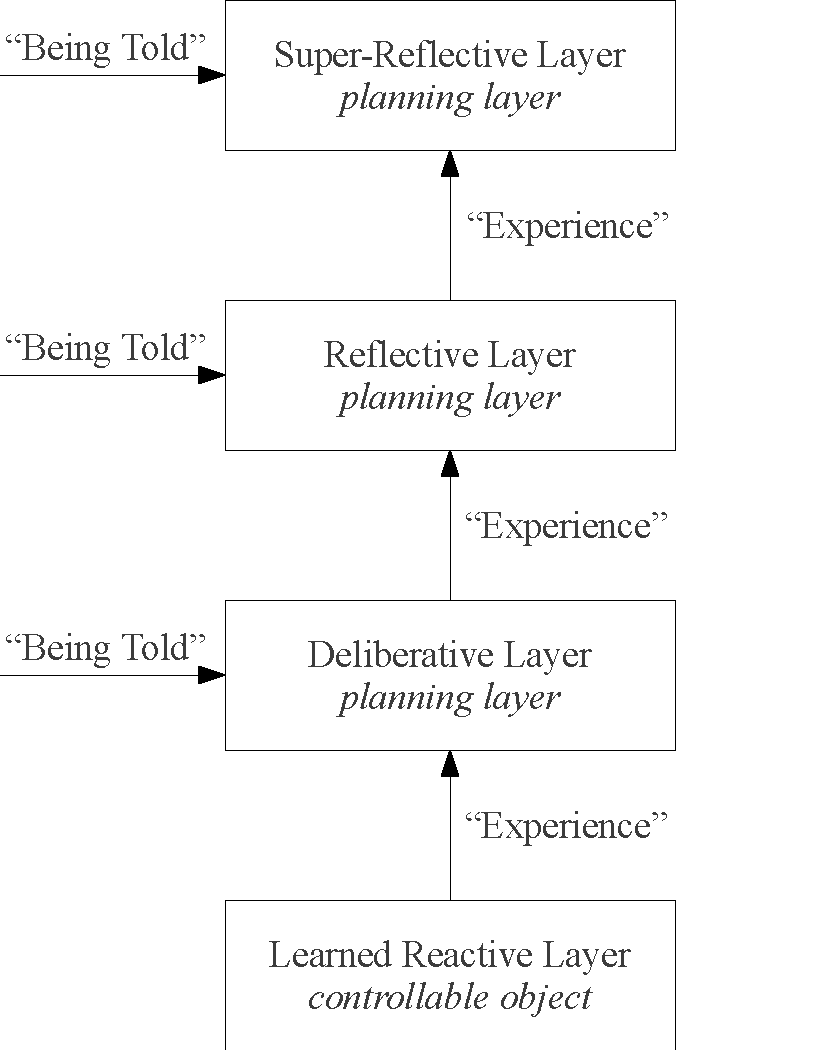
\includegraphics[width=6cm]{gfx/learning_from_being_told_in_layers}
\caption[Learning from being told and learning from experience both
  occur in each SALS planning layer.]{Learning from being told and
  learning from experience both occur in each SALS planning layer.
  When a layer of the AI learns from being told, a natural language
  plan is communicated to that layer from a source external to the AI,
  such as a human user.  When a layer of the AI learns from
  experience, two streams of trace events are received from the layer
  below that are asynchronously woven into hypothetical causal models
  of the effects of actions.}
\label{figure:learning_from_being_told_in_layers}
\end{figure}
In this chapter, I will focus on learning from being told natural
language plans.  I will describe the details of how each planning
layer in SALS asynchronously learns from experience in
{\mbox{\autoref{chapter:learning_asynchronously_from_experience}}}.
The important point that I will elaborate upon in this chapter is that
the SALS AI interprets natural language plans, while simultaneously
considering syntax, semantics, current environmental context, learned
hypothetical knowledge about the effects of actions as well as the
current positive and negative goals of the AI.  My approach is as
opposed to linguistic traditions that focus on only one or two of
these aspects of natural language understanding.

Natural language plans in SALS are in the form of a programming
language with variables, conditionals, recursion, ambiguous values, an
imaginative compiler, and the ability to use analogical patterns
between collections of these plans to interpret natural language
sentences and phrases.  SALS natural language plans are sequences of
commands that can be created, mutated, and executed by a planning
layer to accomplish goals.  The following is an example of a
definition of one of the deliberative plans that the AI in the story
could consider executing:
\begin{samepage}
\begin{Verbatim}
  [defplan 'move left'
    [call-below 'move left']]
\end{Verbatim}
\end{samepage}
This expression defines a new deliberative plan.  The
``{\tt{defplan}}'' command is shorthand for ``define plan.''  The
first argument to the defplan expression is the name of the plan:
``{\tt{move left}}.''  The body of the plan is the remaining sequence
of expressions.  The only expression in the body of this plan is the
``{\tt{call-below}}'' expression with the ``{\tt{move left}}''
argument.  This expression activates a resource in the layer below, in
this case, the ``{\tt{move left}}'' resource, which is in the built-in
reactive layer of the AI.  The ``{\tt{call-below}}'' expression not
only activates a resource in the layer below but also waits for that
resource to complete execution or fail.  The ``{\tt{move left}}'' plan
defines a possible natural language interpretation for the ``{\tt{move
    left}}'' phrase, stating that this phrase refers to the
synchronous execution of the ``{\tt{move left}}'' resource in the
layer below.

Consider this analogous plan to the ``{\tt{move left}}'' plan that
defines an interpretation of the ``{\tt{move right}}'' phrase:
\begin{samepage}
\begin{Verbatim}
  [defplan 'move right'
    [call-below 'move right']]
\end{Verbatim}
\end{samepage}
The analogous similarity between the ``{\tt{move left}}'' and
``{\tt{move right}}'' commands can be abstracted into a new
``{\tt{move left}}'' natural language plan that uses the following
syntax:
\begin{samepage}
\begin{Verbatim}
  [defplan 'move left'
    :matches ['move [? direction]']
     :frame [[direction 'left']]
      [call-below 'move [? direction]']]
\end{Verbatim}
\end{samepage}
This generalized form of the original ``{\tt{move left}}'' and
``{\tt{move right}}'' plans uses a natural language variable,
``{\tt{direction}}.''  Note that there are two optional arguments to
the defplan expression in this example: (1) ``{\tt{:matches}}'' and
(2) ``{\tt{:frame}}.''  The optional ``{\tt{:matches}}'' argument
specifies a list of potential natural language patterns that this plan
may match as it is being interpreted.  In this case, the variable
expression ``{\tt{[?  direction]}}'' is allowed to replace the word
``{\tt{left}}'' from the original name of the plan.  The optional
``{\tt{:frame}}'' argument specifies the default natural language
variable bindings.  In this case, the ``{\tt{direction}}'' variable is
assigned the natural language phrase ``{\tt{left}}'' by default.  In
the body of the generalized form of the plan, all occurrences of
``{\tt{left}}'' have been replaced with the variable expression
``{\tt{[?  direction]}}''.  Given this generalized form of the
original plan, the planner can create a new analogous plan as an
interpretation of either of the natural language phrases: ``{\tt{move
    left}}'' or ``{\tt{move right}}.''

\section{Conditionals and Partial States}

The SALS natural planning language includes conditional branches that
can change the course of plan execution based on the existence of
partial states in the knowledge base that it is trying to control.
For example, here is a more complicated SALS plan that shows a number
of new SALS primitives that will be discussed next:
\begin{samepage}
\begin{Verbatim}
  [defplan 'move toward a cube'
    [if [exists [relationship block property shape cube
	                      preposition left-of
	                      gripper property is-me true]]
        [call-below 'move left']
      [if [exists [relationship block property shape cube
                                preposition right-of
                                gripper property is-me true]]
          [call-below 'move right']
        [fail]]]]
\end{Verbatim}
\end{samepage}
This plan checks to see if there is a cube to the left of the gripper
that the AI is controlling.  If there is a cube to the left, this plan
will activate the ``{\tt{move left}}'' resource in the layer below.
If there is not a cube to the left, this plan then checks to see if
there is a cube to the right of the gripper that the AI is
controlling.  If there is a cube to the right, this plan will activate
the ``{\tt{move right}}'' resource in the layer below.  At this point,
if there is not a cube to the left or to the right, the plan fails.
There are a number of new primitives that are introduced in this
example of conditional branches:
\begin{packed_itemize}
\item{``{\tt{if}}''}
\item{``{\tt{exists}}''}
\item{``{\tt{relationship}}''}
\item{``{\tt{fail}}''}
\end{packed_itemize}
The syntax for the SALS ``{\tt{if}}'' expression is similar to the
``{\tt{if}}'' expression in most lisp-like languages: the first
argument is the conditional, the second argument is the true branch,
and the remaining arguments are the optional body of the false branch.
Unlike most lisp-like languages, the SALS ``{\tt{if}}'' expression's
conditional value must be a Boolean type object and will fail with any
other value.  The ``{\tt{fail}}'' expression is a simple way for a
plan to stop executing and mark the plan with the knowledge of a
failure object.  The ``{\tt{exists}}'' expression accepts a partial
state as its only argument and checks to see if this partial state
exists in the knowledge base that the planning layer is trying to
control.  When the effects of a plan are being imagined, the return
value of the ``{\tt{exists}}'' expression are not known, so multiple
possible ambiguous values are returned: (1) the result based on
current hypothetical models of the effects of previous actions or the
current state of the knowledge base that this planning layer is trying
to control if no previous actions have been imagined, (2) a true value
based on the possibility that learned models are incorrect, and (3) a
false value based on the possibility that learned models are
incorrect.  The ``{\tt{relationship}}'' expression is one of two
special expressions in SALS that return partial state objects.  The
``{\tt{relationship}}'' expression accepts ten arguments, which map
directly to the internal semantic graph representation of the
knowledge base that the planning layer is trying to control.  The
following are the ten arguments to the ``{\tt{relationship}}''
expression:
\begin{packed_enumerate}
\item{{\tt{source-type}}}
\item{{\tt{source-key-type}}}
\item{{\tt{source-key}}}
\item{{\tt{source-value}}}
\item{{\tt{key-type}}}
\item{{\tt{key}}}
\item{{\tt{target-type}}}
\item{{\tt{target-key-type}}}
\item{{\tt{target-key}}}
\item{{\tt{target-value}}}
\end{packed_enumerate}
{\mbox{\autoref{figure:relationship_partial_state_graph}}} shows how
the arguments to the ``{\tt{relationship}}'' expression map to the
frame types, slot values, and properties of a frame-based knowledge
base that is represented as a graph.  When an argument to the
``{\tt{relationship}}'' expression is a symbol, this symbol is checked
against a list of known symbols within the SALS AI.  If an argument to
the ``{\tt{relationship}}'' expression is not a known symbol, this
results in an interpretation failure, limiting the number of possible
interpretations.
\begin{figure}
\centering
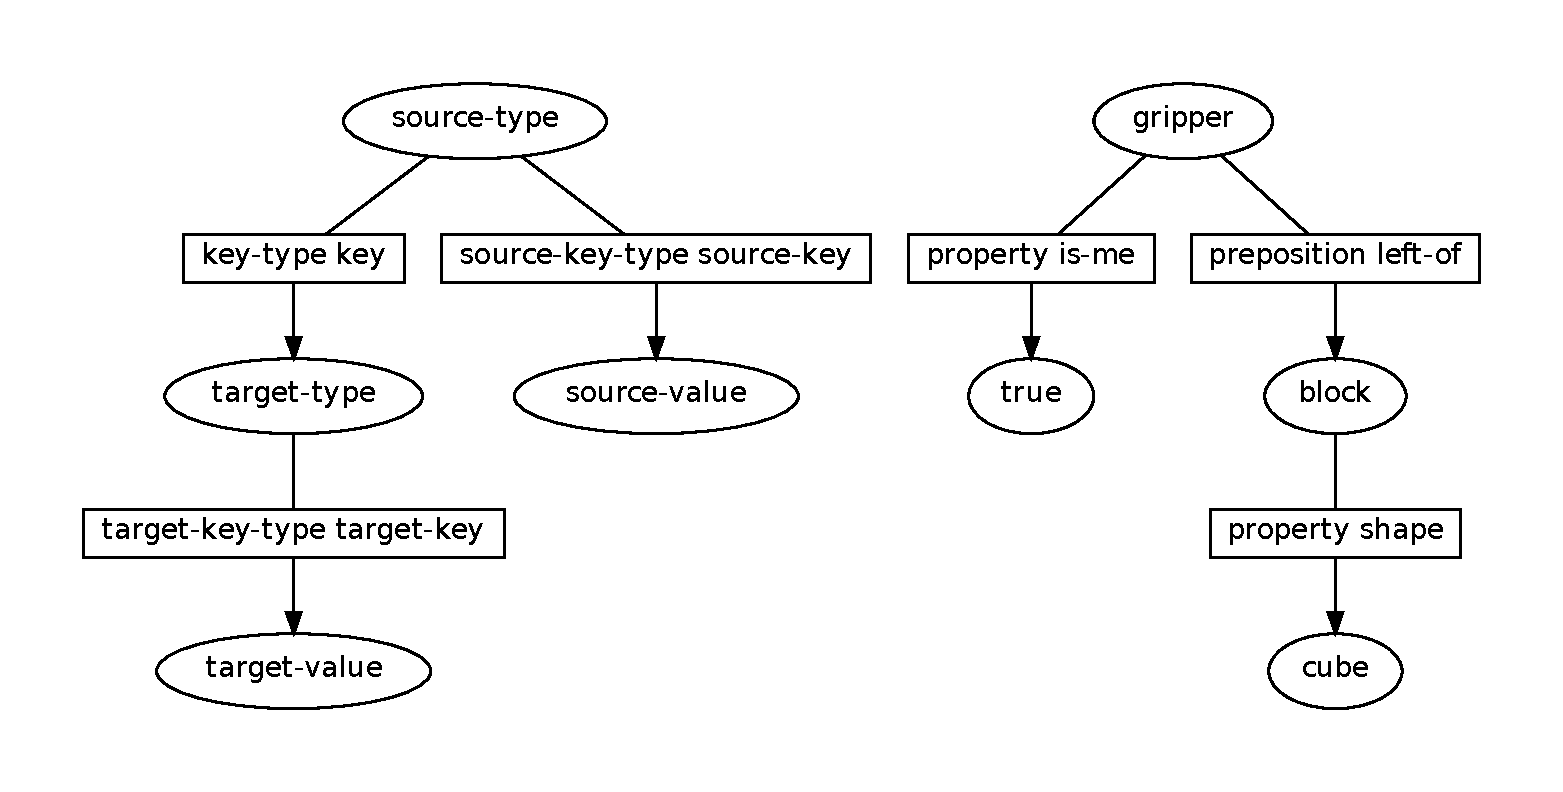
\includegraphics[width=12cm]{gfx/relationship_partial_state_graph}
\caption[The SALS ``{\tt{relationship}}'' expression returns a partial
  state object.]{The SALS ``{\tt{relationship}}'' expression returns a
  partial state object.  The graph on the left shows the ten argument
  names for the ``{\tt{relationship}}'' expression, while the graph on
  the right shows a potential partial state of the physical knowledge
  base that literally means, ``{\tt{a cube shaped block to be to the
      left of a gripper that is me}}.''}
\label{figure:relationship_partial_state_graph}
\end{figure}

Now, let us consider a slightly different type of partial state
expression in the following example plan that attempts to control the
gripper to grab a block:
\begin{samepage}
\begin{Verbatim}
  [defplan 'attempt to grab block'
    [call-below 'grab']
    [wait-for [property gripper property is-me true
                        property movement-command
                        stop]]]
\end{Verbatim}
\end{samepage}
In this plan, two new types of SALS expressions are introduced:
\begin{packed_itemize}
\item{``{\tt{wait-for}}''}
\item{``{\tt{property}}''}
\end{packed_itemize}
The ``{\tt{wait-for}}'' expression takes one argument, which similarly
to the ``{\tt{exists}}'' expression, must be a partial state object,
such as that returned by the ``{\tt{relationship}}'' expression.
Functionally, the ``{\tt{wait-for}}'' expression puts the plan to
sleep until the specified partial state exists in the knowledge base
in the layer below that this plan is trying to control.  The
``{\tt{property}}'' expression is similar to the
``{\tt{relationship}}'' expression in that it does return a partial
state object, but the ``{\tt{property}}'' expression only takes the
following seven arguments:
\begin{packed_enumerate}
\item{{\tt{source-type}}}
\item{{\tt{source-key-type}}}
\item{{\tt{source-key}}}
\item{{\tt{source-value}}}
\item{{\tt{key-type}}}
\item{{\tt{key}}}
\item{{\tt{value}}}
\end{packed_enumerate}
{\mbox{\autoref{figure:relationship_partial_state_graph}}} shows how
the arguments to the ``{\tt{property}}'' expression map to the frame
types, slot values, and properties of a frame-based knowledge base
that is represented as a graph.
\begin{figure}
\centering
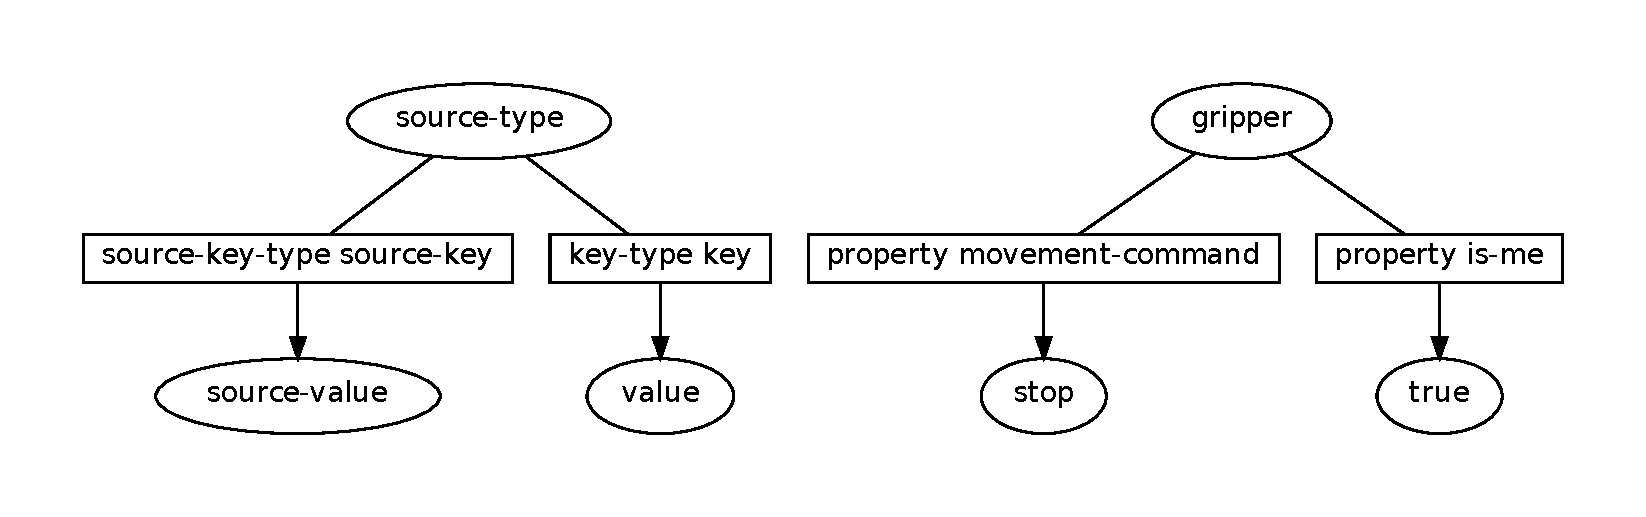
\includegraphics[width=12cm]{gfx/property_partial_state_graph}
\caption[The SALS ``{\tt{property}}'' expression returns a partial
  state object.]{The SALS ``{\tt{property}}'' expression returns a
  partial state object.  The graph on the right shows the seven
  argument names for the ``{\tt{property}}'' expression, while the
  graph on the left shows a potential partial state of the physical
  knowledge base that literally means, ``{\tt{a gripper to be me and
      have a stop movement command}}.''}
\label{figure:property_partial_state_graph}
\end{figure}

While the deliberative layer may create plans that refer to partial
states in the physical knowledge base, the reflective layer may create
plans that refer to partial states in the deliberative plan knowledge
base, which may in turn also refer to partial states in the physical
knowledge base.  Consider the following example of a reflective plan
that includes this form of hierarchical partial state reference:
\begin{samepage}
\begin{Verbatim}
  [defplan 'a deliberative planner to have a positive goal
            for a cube to be on a pyramid'
    [property planner property layer deliberative
              property positive-goal
              [relationship block property shape cube
                            preposition on
                            block property shape pyramid]]]
\end{Verbatim}
\end{samepage}
In this reflective plan, the ``{\tt{property}}'' expression describes
a partial state of the deliberative plan knowledge base, while the
``{\tt{relationship}}'' expression describes a partial state of the
physical knowledge base.  For SALS to convert this expression to a
purely deliberative form of knowledge, hierarchical partial states are
reified in SALS so that they become a simple partial state that is
purely of one layer's type of knowledge.  When a partial state object
is passed as an argument to another partial state object, the first
partial state is converted to a symbolic form, so that the entire
structure can continue to exist as a simple frame-based graph
structure.  {\mbox{\autoref{figure:hierarchical_partial_state_graph}}}
shows an example of a hierarchical embedding of
``{\tt{relationship}}'' and ``{\tt{property}}'' partial states that
may occur in any planning layer above the deliberative layer.
\begin{figure}
\centering
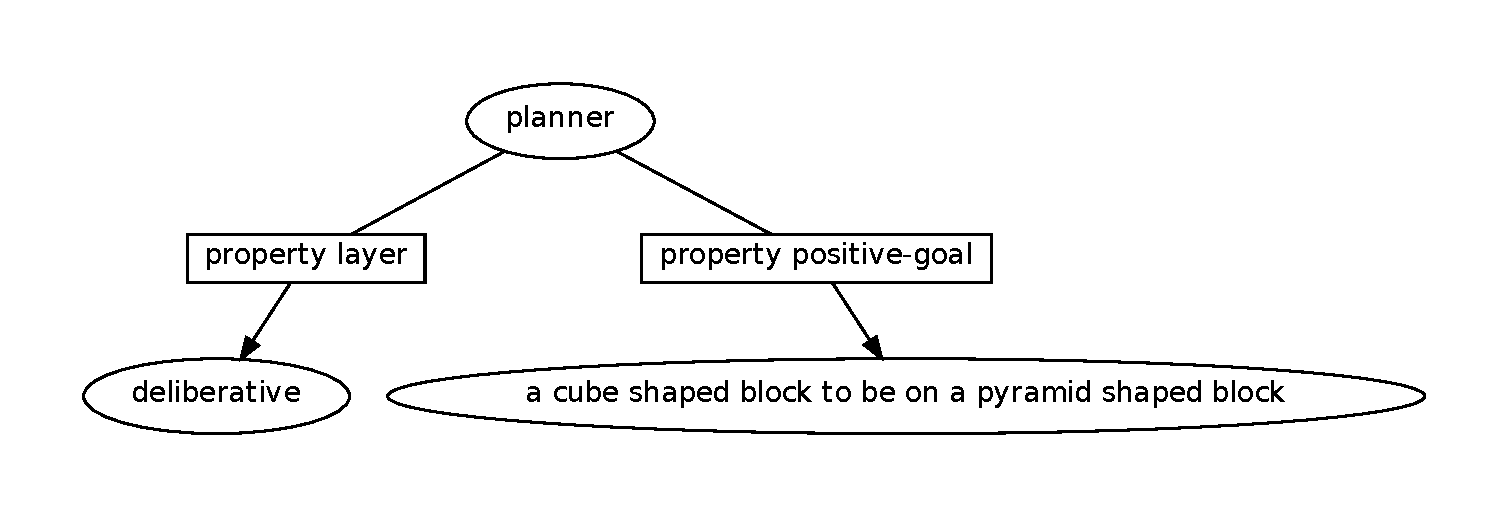
\includegraphics[width=12cm]{gfx/hierarchical_partial_state_graph}
\caption[The SALS ``{\tt{relationship}}'' and ``{\tt{property}}''
  expressions can be hierarchically combined in planning layers above
  the deliberative.]{The SALS ``{\tt{relationship}}'' and
  ``{\tt{property}}'' expressions can be hierarchically combined in
  planning layers above the deliberative.  Note that any partial
  states that are sub-expressions of other partial states become
  symbolically reified to maintain a frame-based graph structure for
  all knowledge.}
\label{figure:hierarchical_partial_state_graph}
\end{figure}

\section{Plans Interpreting Plans}
\label{section:plans_interpreting_plans}

The most powerful capability of the SALS natural language programming
language is the ability to find correct interpretations of ambiguous
natural language plans.  Let us first define the following simple
natural language plan that returns a ``{\tt{relationship}}'' partial
state object:
\begin{samepage}
\begin{Verbatim}
  [defplan 'a cube to be to my left'
    [relationship block property shape cube
                  preposition left-of
                  gripper property is-me true]]
\end{Verbatim}
\end{samepage}
This plan can be generalized to analogously work for any type of shape
as in the following example:
\begin{samepage}
\begin{Verbatim}
  [defplan 'a cube to be to my left'
    :matches ['a [? shape] to be to my left']
     :frame [[shape 'cube']]
      [relationship block property shape [? shape]
                    preposition left-of
                    gripper property is-me true]]
\end{Verbatim}
\end{samepage}
Now, consider the following plan that makes use of this previous plan
definition and introduces two new SALS expression types for evaluating
natural language plans:
\begin{samepage}
\begin{Verbatim}
  [defplan 'a cube is to my left'
    [exists [plan-call [plan 'a cube to be to my left']]]]
\end{Verbatim}
\end{samepage}
This last plan returns a true or false value depending on whether or
not the partial state returned by the plan, ``{\tt{a cube to be to my
    left}},'' exists in the knowledge base that the planning layer is
trying to control.  Two new types of SALS natural language programming
expressions are introduced in the last plan:
\begin{packed_enumerate}
\item{``{\tt{plan-call}}''}
\item{``{\tt{plan}}''}
\end{packed_enumerate}
The ``{\tt{plan}}'' expression takes one argument, a natural language
phrase.  The ``{\tt{plan}}'' expression returns a plan from the
current planning layer that matches the given natural language phrase.
If there is no matching natural language plan, SALS will attempt to
find an plan that has an analogous match to the given natural language
phrase.  In most cases, there are multiple possible matches for any
given natural language phrase.  In these cases, the SALS natural
language plan compiler is responsible for imagining the effects of
different interpretations on the knowledge base that the planning
layer is trying to control, while avoiding natural language plan
interpretation failures.  The ``{\tt{plan-call}}'' expression accepts
one argument, a natural language subplan to compile into this location
of the current plan that is being defined by the ``{\tt{defplan}}''
expression.

Now, consider the following redefinition of the previous ``{\tt{move
    toward a cube}}'' plan that I defined previously:
\begin{samepage}
\begin{Verbatim}
  [defplan 'move toward a cube'
    [if [plan-call [plan 'a cube is to my left']]
        [call-below 'move left']
      [if [plan-call [plan 'a cube is to my right']]
          [call-below 'move right']
        [fail]]]]
\end{Verbatim}
\end{samepage}
This version of the ``{\tt{move toward a cube}}'' natural language
plan is simpler because it only indirectly references the
``{\tt{relationship}}'' and ``{\tt{exists}}'' expressions through the
``{\tt{plan}}'' and ``{\tt{plan-call}}'' expressions that refer to the
appropriate analogies to other natural language plans.  Now, consider
the following expression that defines an analogy for any natural
language plans that use the ``{\tt{if}}'' expression:
\begin{samepage}
\begin{Verbatim}
  [defplan 'if a cube is to my left, move left,
            otherwise move right'
    :matches ['if [? condition], [? true-branch],
               otherwise [? false-branch]']
     :frame [[condition    'a cube is to my left']
             [true-branch  'move left']
             [false-branch 'move right']]
      [if [plan-call [plan [? condition]]]
          [plan-call [plan [? true-branch]]]
        [plan-call [plan [? false-branch]]]]]
\end{Verbatim}
\end{samepage}
Using this definition of an analogy for the ``{\tt{if}}'' expression,
the original ``{\tt{move toward a cube}}'' natural language plan can
be rewritten as follows:
\begin{samepage}
\begin{Verbatim}
  [defplan 'move toward a cube'
    [plan-call [plan 'if a cube is to my left, move
                      left, otherwise if a cube is
                      to my right, move right,
                      otherwise fail']]]
\end{Verbatim}
\end{samepage}
Note that this last plan uses two ``{\tt{if}}'' statements, the second
is in the false branch of the first.

Before getting to the details of how ambiguity in searched through and
eliminated in the SALS natural language plan compiler, consider the
following definitions that include the SALS ``{\tt{not}}'' expression:
\begin{samepage}
\begin{Verbatim}
  [defplan 'a cube is not to my left'
    [not [plan-call [plan 'a cube is to my left']]]]
\end{Verbatim}
\end{samepage}
The SALS ``{\tt{not}}'' expression is similar to the ``{\tt{not}}''
expression in most lisp-like programming languages in that it takes
one argument.  Unlike most lisp-like languages, the SALS
``{\tt{not}}'' expression only accepts a Boolean type of object.  The
``{\tt{not}}'' expression returns a new Boolean type object that
represents the opposite value of the argument.  The following is an
analogous plan that can be used to generalize this natural language
usage of the ``{\tt{not}}'' expression:
\begin{samepage}
\begin{Verbatim}
  [defplan 'a cube is not to my left'
    :matches ['[? subject] is not [? preposition]']
     :frame [[subject     'a cube']
             [preposition 'to my left']]
      [not [plan-call [plan '[? subject] is
                             [? preposition]']]]]
\end{Verbatim}
\end{samepage}
This plan allows many negative expressions to analogously have a
correct interpretation, such as ``{\tt{if a pyramid is not to my
    right, move left, otherwise fail}}.''

Another powerful component of the SALS natural programming language is
the ability to compile natural language plans that include recursive
references, which enable plans to describe looping functionality.
SALS also has a primitive capability to imagine the possible effects
of loops by imaginatively unrolling the loop only once.  The following
example is a definition of a reflective natural language plan that
searches for a deliberative plan whose effects have not yet been
imagined:
\begin{samepage}
\begin{Verbatim}
  [defplan 'find next unimagined plan'
    [call-below 'focus on next object']
    [plan-call [plan 'if a planner is focusing on
                      a plan that has been imagined,
                      find next unimagined plan']]]
\end{Verbatim}
\end{samepage}
Notice that the name of this plan is ``{\tt{find next unimagined
    plan}},'' which is the same as the true branch of the natural
language ``{\tt{if}}'' statement in the body of the plan.  This plan
checks to see if the plan currently in the focus of the deliberative
planner has been imagined.  If the plan in deliberative focus has been
imagined, this plan calls itself recursively until the deliberative
planner is focusing on a plan that has not been imagined.

As a final example of a natural language plan interpreting a natural
language plan, consider again the following hierarchical partial state
construction from a reflective natural language plan from earlier in
this chapter:
\begin{samepage}
\begin{Verbatim}
  [defplan 'a deliberative planner to have a positive goal
            for a cube to be on a pyramid'
    [property planner property layer deliberative
              property positive-goal
              [relationship block property shape cube
                            preposition on
                            block property shape pyramid]]]
\end{Verbatim}
\end{samepage}
This reflective natural language plan can be abstracted with
``{\tt{plan}}'' and ``{\tt{plan-call}}'' expressions as in the
following example:
\begin{samepage}
\begin{Verbatim}
  [defplan 'a deliberative planner to have a positive goal
            for a cube to be on a pyramid'
    :matches ['a deliberative planner to have a positive
               goal for [? partial-state]']
     :frame [[partial-state 'a cube to be on a pyramid']]
      [property planner property layer deliberative
                property positive-goal
                [plan-call [plan [? partial-state]]]]]
\end{Verbatim}
\end{samepage}
In this way, analogous reflective plans can be created to allow the
interpretation of any natural language physical partial state being a
positive goal of the deliberative planning layer.  A similar technique
can be used to create analogous reflective natural language plans that
work for negative goals as well as plans that are hypothesized to
cause partial states to exist.

\section{Analogous Plan Interpretation}

As previously described, the ``{\tt{plan}}'' expression in a SALS
natural language plan returns a plan object that either matches the
name of a plan previously defined via the ``{\tt{defplan}}''
expression, or if an analogy can be found to an existing plan, a new
analogous plan object is created and returned as the result of the
``{\tt{plan}}'' expression.  Because of the possibility that multiple
plans may match a given ``{\tt{plan}}'' expression, it is the task of
the SALS compiler to imagine the effects of the different
interpretations and decide upon one for execution.  The SALS natural
language plan compiler must handle multiple ambiguous return values
for each ``{\tt{plan}}'' expression.  Let us consider again the
following natural language plan that must be imagined and interpreted,
which requires the compiler to sort through multiple possible
interpretations:
\begin{Verbatim}
  [plan-call [plan 'if a cube is not on a pyramid, stack a
                    cube on a pyramid']]
\end{Verbatim}
A reasonable way to expect this natural language phrase to be
interpreted is as a plan analogous to the natural language plan for
the ``{\tt{if}}'' expression similar to the one previously defined, as
in the following:
\begin{samepage}
\begin{Verbatim}
  [defplan 'if a cube is not on a pyramid, stack a cube on a
            pyramid'
    :matches ['if [? condition], [? true-branch]']
     :frame [[condition    'a cube is not on a pyramid']
             [true-branch  'stack a cube on a pyramid']]
      [if [plan-call [plan [? condition]]]
          [plan-call [plan [? true-branch]]]]]
\end{Verbatim}
\end{samepage}
Although this plan makes sense, there are many other possible
problematic analogies to previously defined natural language plans
that do not make any sense at all.  The following problematic
interpretation is one example:
\begin{samepage}
\begin{Verbatim}
  [defplan 'if a cube is not on a pyramid, stack a cube on a
            pyramid'
    :matches ['[? subject] is not [? preposition]']
     :frame [[subject     'if a cube']
             [preposition 'on a pyramid, stack a cube on a
                           pyramid']]
      [not [plan-call [plan '[? subject] is
                             [? preposition]']]]]
\end{Verbatim}
\end{samepage}
Notice that the natural language value of the ``{\tt{subject}}''
variable in the previous problematic interpretation is equal to
``{\tt{if a cube}}.''  The following is the result of one step in
compiling this problematic interpretation:
\begin{Verbatim}
  [not [plan-call [plan 'if a cube is on a pyramid, stack a
                         cube on a pyramid']]]
\end{Verbatim}
Notice that the ``{\tt{not}}'' expression has been moved to the front
of this expression after it has been partially compiled.  The
following is the result of another couple steps of further
interpreting the remaining natural language in this expression:
\begin{Verbatim}
  [not [if [exists [plan-call [plan 'a cube to be on a
                                     pyramid']]]
           [plan-call [plan 'stack a cube on a pyramid']]]]
\end{Verbatim}
When this problematic interpretation is imagined, the result from the
``{\tt{exists}}'' expression is a Boolean value, so this satisfies the
``{\tt{if}}'' conditional type requirement.  However, the result of
the ``{\tt{if}}'' expression is the special type ``{\tt{nil}},'' which
is not a Boolean value in the SALS natural programming language.
Because the ``{\tt{not}}'' expression strictly requires a Boolean type
value, the imaginative interpretation of this plan fails when the nil
value from the ``{\tt{if}}'' statement reaches the ``{\tt{not}}''
expression.  Using strict typing in the low-level details of the SALS
natural programming language allows ambiguous high-level expressions
with many possible interpretations to be narrowed down to a few that
make programmatic sense.  By introducing more constraints to the
low-level details of the SALS natural programming language, many types
of plan failures can be imagined and avoided, even while using this
very loose type of natural language analogical matching technique.
Not all errors can be imagined and avoided through imaginative
compiling, but many types of failures are avoided in this way.
However, some failures, such as expectation failures, can only be
realized during the actual execution of the plan.

\section{Imagining the Effects of Ambiguous Plans}
\label{section:imagining_the_effects_of_ambiguous_plans}

As natural language plans are interpreted, the hypothetical effects of
any resource activations in the layer below are also simultaneously
imagined in the counterfactual knowledge base of that planning layer.
Imagining the effects of resource activations first requires that
hypothetical models of the effects of resource activations exist.
Hypothetical models of the effects of resource activations in SALS
provide a rule-based mapping from the preconditions of the resource
activation to the potential transframes for the resource activation.
The preconditions and transframes are in terms of the abstract partial
states that have previously existed in the knowledge base that the
planning layer is trying to control.  For example, ``{\tt{a gripper
    that is me being above a cube shaped block}}'' could be one of
many preconditions for an action.  All partial states that can be
returned by the ``{\tt{relationship}}'' and ``{\tt{property}}''
expressions in the SALS natural programming language are efficiently
abstracted asynchronously from the knowledge base that the planning
layer is trying to control.  I will describe the details of the
abstract asynchronous learning algorithm for each planning layer in
{\mbox{\autoref{chapter:learning_asynchronously_from_experience}}}.
For now, know that abstract hypothetical models of resource
activations are learned and can be used for imagining the effects of
resource activations during the natural language plan interpretation
process.

Because some expressions in the SALS natural planning language can
return multiple possible ambiguous values, one task of the planning
layer is to decide which of the multiple possible interpretations is
complete, accomplishes positive goals and avoids negative goals.  This
means that each expression in the SALS natural programming language
may have one or more possible different outcomes, depending on the
interpretation path and which one of potentially multiple ambiguous
values is chosen to be executed when a decision must be made.  In
order to keep track of each of these different interpretations, each
plan expression is allocated an {\emph{execution node}} object and
each decision among multiple ambiguous argument values is allocated an
{\emph{argument decision node}} object in the plan knowledge base of
that planning layer.  The execution node objects correspond to the
functional hierarchy of the imagined natural language plan execution,
while the argument decision node objects represent any points in the
imagined execution where two potentially different sub-trees of the
functional execution could occur based on different choices between
multiple possible ambiguous return values from sub-expressions of the
current expression being imaginatively executed.
\begin{figure}
\hspace*{-1cm}\includegraphics[width=14cm]{gfx/plan_execution_node_graph}
\caption[A graph representation of the deliberative plan knowledge
  base while a simple plan with multiple ambiguous interpretations is
  being imaginatively interpreted and evaluated.]{A graph
  representation of the deliberative plan knowledge base while a
  simple plan with multiple ambiguous interpretations is being
  imaginatively interpreted and evaluated.  The deliberative
  {\emph{planner}} object is focusing on a {\emph{plan}} object that
  has been partially evaluated.  The first execution node object of
  this plan object represents the partial interpretation of a
  ``{\tt{not}}'' expression that has a ``{\tt{plan-call}}''
  sub-expression.  The ``{\tt{plan}}'' expression returns two possible
  values, which are interpreted separately under argument decision
  node objects.}
\label{figure:plan_execution_node_graph}
\end{figure}
{\mbox{\autoref{figure:plan_execution_node_graph}}} shows a graph
representation of the frame-based deliberative plan knowledge base as
it is in the process of imaginatively evaluating the following simple
plan:
\begin{samepage}
\begin{Verbatim}
  [defplan 'a cube is not on a pyramid'
    :matches ['[? subject] is not [? preposition]']
     :frame [[subject     'a cube']
             [preposition 'on a pyramid']]
      [not [plan-call [plan '[? subject] is
                             [? preposition]']]]]
\end{Verbatim}
\end{samepage}
When this natural language plan is imaginatively interpreted, there
are multiple possible values returned from the ``{\tt{plan}}''
expression, which returns analogous plans that match the natural
language phrase, ``{\tt{a cube is on a pyramid}}.''  In this case,
there are the two following plans that are created as analogies to
other known plans:
\begin{packed_enumerate}
\item{
\begin{samepage}
\begin{Verbatim}
  [defplan 'a pyramid is on a cube'
    :matches ['a [? top-shape] is on a [? bottom-shape]']
     :frame [[top-shape    'pyramid']
             [bottom-shape 'cube']]
      [exists [relationship block property shape
                              [? top-shape]
                            preposition on
                            block property shape
                              [? bottom-shape]]]]
\end{Verbatim}
\end{samepage}
}
\item{
\begin{samepage}
\begin{Verbatim}
  [defplan 'a pyramid is on a cube'
    :matches ['a [? top-color] is on a [? bottom-color]']
     :frame [[top-color    'pyramid']
             [bottom-color 'cube']]
      [exists [relationship block property color
                              [? top-color]
                            preposition on
                            block property color
                              [? bottom-color]]]]
\end{Verbatim}
\end{samepage}
}
\end{packed_enumerate}
The first of these two analogous interpretations is what one would
expect: the natural language phrases ``{\tt{pyramid}}'' and
``{\tt{cube}}'' are interpreted to be shapes of blocks that are on top
of one another.  The second of these interpretations is less obvious
and incorrectly interprets ``{\tt{pyramid}}'' and ``{\tt{cube}}'' to
be colors.  This problematic interpretation is an analogy to the
following plan that the SALS AI already knows:
\begin{samepage}
\begin{Verbatim}
  [defplan 'a red is on a blue'
    :matches ['a [? top-color] is on a [? bottom-color]']
     :frame [[top-color    'red']
             [bottom-color 'blue']]
      [exists [relationship block property color
                              [? top-color]
                            preposition on
                            block property color
                              [? bottom-color]]]]
\end{Verbatim}
\end{samepage}
The SALS AI does not immediately know that ``{\tt{red}}'' and
``{\tt{blue}}'' are colors, while ``{\tt{cube}}'' and
``{\tt{pyramid}}'' are shapes.  While types of partial states could be
programmed into the SALS AI so that these specific words could be
assigned specific symbolic types, this is not the approach taken in
the SALS AI.  Instead, both of these interpretations are plausible in
the SALS AI.  However, when the SALS AI does finish imagining all
possible interpretations of a natural language phrase, each different
resulting analogous plan has a set of associated hypothetical states
that this plan may or may not accomplish.  If the possible effects of
a plan include a ``{\tt{pyramid}}'' color, which does not make sense,
the SALS AI sees that this is not one of its goals, so it ignores this
interpretation for that reason alone.  The SALS AI is a goal-oriented
natural language understanding system in this sense---finding those
natural language plan interpretations that it thinks will accomplish
its positive goals.  On the other hand, the SALS AI considers its
negative goals in the opposite sense: when a natural language plan
interpretation is hypothesized to accomplish a negative goal, that
plan interpretation is ignored.  The SALS AI can be considered to be
an ``optimistic'' or ``pessimistic'' natural language understanding
system in these cases.  The important point here is that the SALS AI
interprets natural language plans, while simultaneously considering
syntax, semantics, current environmental context, learned hypothetical
knowledge about the effects of actions as well as the current positive
and negative goals of the AI.

There are two ways that a natural language plan is hypothesized to
cause a specific partial state: (1) learned hypothetical models are
used to predict the effects of actions, and (2) existence checks for
partial states during the imaginative interpretation of the plan are
used as secondary evidence that a plan may or may not be expecting a
specific partial state to exist during its execution.  For example, if
a natural language plan checks for the existence of the partial state,
``{\tt{a cube shaped block to be on top of a pyramid shaped block}},''
this existence check provides secondary evidence that this plan could
be expecting this state to exist during its execution.  This secondary
evidence of the possible intentions of a plan is an example of
knowledge learned during the imaginative interpretation of natural
language plans in the SALS AI.

